\begin{figure}[h!]
\textbf{Tema d'Esame di Gennaio 2015}\\ \\
Si determini la differenza di potenziali ai capi della resistenza $R4$ del circuito mostrato in figura. La differenza di potenziale fornita dalla batteria è di $12V$ e i valori delle resistenze sono rispettivamente $R2=15\Omega, R3=40\Omega, R4=24\Omega, R5=R6=32\Omega, R1=R7=18\Omega$
\begin{center}
		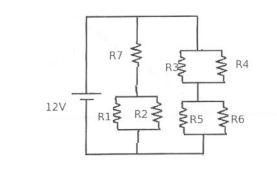
\includegraphics[scale=1.2]{ES5/GEN052015.jpg}
	\end{center}
\end{figure}

\begin{figure}[h!]
\textbf{Tema d'Esame di Febbraio 2015}\\ \\
 Nel circuito in figura, la corrente attraverso $R6$ è $i_6=1.40A$ e le resistenze sono
$R1=R2=R3=2.0\Omega, R4= 16.0\Omega, R5= 8.0 \Omega e R6= 4.0 \Omega$. Qual'è la forza elettromotrice della batteria (ideale)?
\begin{center}
		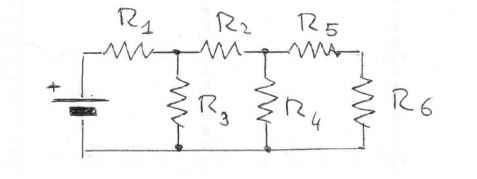
\includegraphics[scale=0.8]{ES5/FEB052015.jpg}
	\end{center}
\end{figure}

\begin{figure}[h!]
\textbf{Tema d'Esame di Giugno 2015}\\ \\
Si determini la differenza di potenziali ai capi della resistenza R4 del circuito mostrato in figura. La differenza di potenziale fornita dalla batteria è di $12V$ e i valori delle resistenze sono rispettivamente $R2=15\Omega, R3=40\Omega, R4=25\Omega, R5=R6=32\Omega, R1=R7=18\Omega$.
\begin{center}
		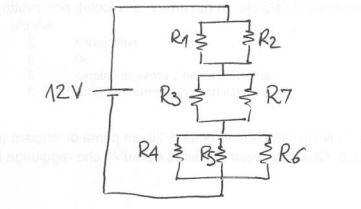
\includegraphics[scale=1]{ES5/GIU052015.jpg}
	\end{center}
\end{figure}

\begin{figure}[h!]
\textbf{Tema d'Esame di Luglio 2015}\\ \\
La differenza di potenziale fornita dalla batteria è di $12V$ e i valori delle resistenze sono rispettivamente $R2=15\Omega, R3=40\Omega, R4=25\Omega, R5=R6=32\Omega, R1=R7=18\Omega$
\begin{center}
		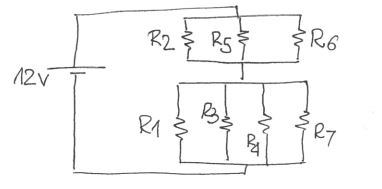
\includegraphics[scale=1]{ES5/LUG052015.jpg}
	\end{center}
\end{figure}